\chapter{刀具磨损预测模型搭建}
% 
% 
% 
% 
\section{基于神经网络的刀具磨损量测定模型}
我们试图寻找一种可以在机床工作时也可以测定刀具磨损度的预测方法,我们先对高维信号进行特征工程处理,在此基础上,将所获得的特征值与一维数据结合,运用Recurrent Neural Network循环神经网络模型对刀具磨损量进行预测。\par
% 
\begin{figure}[htp]
    \centering
    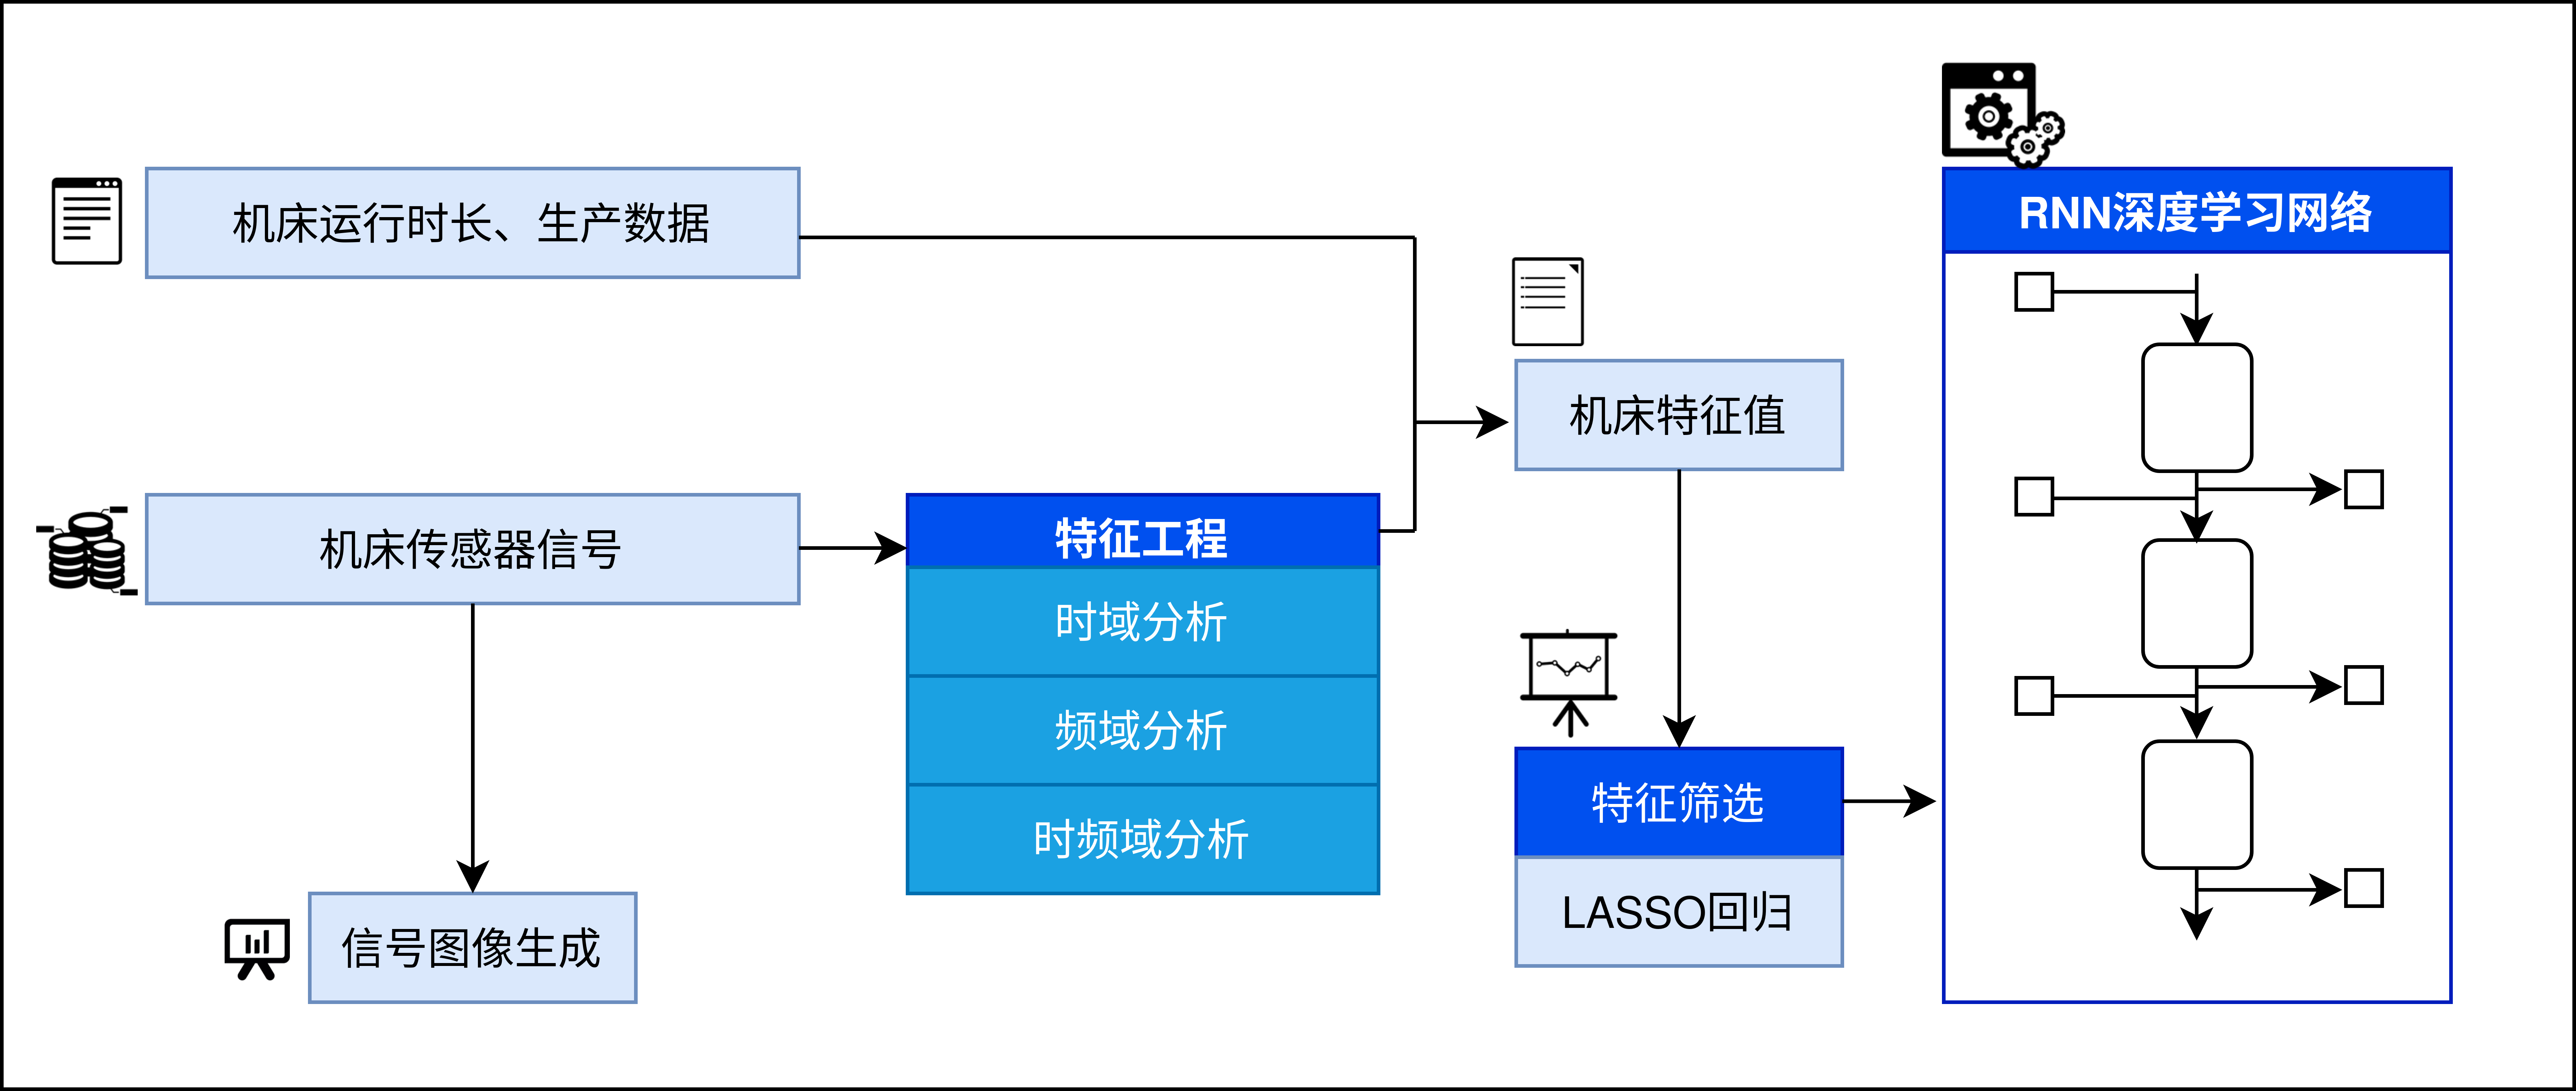
\includegraphics[width=14cm]{Chapter2/RNN测定模型.png}
    \caption{刀具磨损预测流程图}
\end{figure}
% 
\subsection{模型输入数据类型}
我们所用的数据来源于松浦MC-510V加工中心的具体操作数据。\par
% 
% 
% 
在操作过程中,我们采用传感器技术,利用声音传感器、振动传感器、电流传感器对不同操作条件下的铣床运行进行观察与记录,得到了在常规切削、进口切削以及出口切削时的刀具磨损相关数据,并将这些数据实时写入Matlab的mill.mat文件中。\par
% 
% 
在实验操作过程中,铣床上刀具切削的操作条件是从工业适用性角度出发,以制造商推荐的设置为指导,具体如上(见表2.1,2.2)
% 
\begin{table}[]
    \centering
    \caption{数据结构描述介绍}
    \begin{tabular}{c c}
    \hline
    属性 & 描述 \\
    \hline
    切割速度 & 200m/min \to 826r/min \\
    切割深度 & 1.5mm、0.75mm \\
    进给量 & 0.5mm/rev、0.25mm/rev \to 413mm/min、206.5mm/min \\
    材料 & 铸铁、不锈钢J45 \\
    刀片类型 & KC710 \\
    铣床工作台尺寸 &  483mm*178mm*51mm \\
    \hline
    \end{tabular}
\end{table}
% 
% 
\begin{table}[]
    \centering
    \caption{数据结构说明}
    \begin{tabular}{cccc}
        \hline
        符号 & 含义 & 符号 & 含义 \\
        \hline
        case & 案例数量 & smcAC & 主轴交流电信号 \\
        run	& 每个案例中的运行次数 & smcDC & 主轴直流电信号 \\
        VB & 刀具磨损 & vib\_table & 工作台振动信号 \\
        time & 测量时刻 & vib\_spindle & 主轴振动信号 \\
        DOC & 切削深度 & AE\_table & 工作台噪音信号 \\
        feed & 进给量 & AE\_spindle & 主轴噪音信号 \\
        material & 材料 \\
        \hline
    \end{tabular}
\end{table}
% 
% 
% 
% 
\section{特征工程}
\subsection{\href{https://github.com/QianZeHao123/OpenIE/blob/main/nc_machining_center/time_domain_analysis.m}{信号处理}}
特征工程部分MatLab代码: https://github.com/QianZeHao123/OpenIE\\/blob/main/nc\_machining\_center/time\_domain\_analysis.m \par
\subsubsection{时域特征提取}
对于时域特征的提取,我们将有量纲特征值与无量纲特征值相结合,以时间为自变量表示目标信号数据的波形,具体特征如下:\par
% 底下是一堆公式
绝对均值:\par
$$ |\bar{x}|=\frac{1}{N} \sum_{i=1}^{N}\left|x_{i}\right| $$\par
峰值:\par
$$ x_{pesk}=X_{max} $$\par
均方根值:\par
$$ x_{rms}=\sqrt{\frac{1}{N} \sum_{k=1}^{N} x_{i}^{2}} $$\par
方根幅值:\par
$$ x_{kurtosis}=\frac{1}{N} \sum_{k=1}^{N}(\pi)^{n} $$\par
峭度值:\par
$$ x_{ra}=\left(\frac{1}{N} \sum_{i=1}^{N} \sqrt{|x_i|}\right)^{2} $$\par
波形因子:\par
$$ f_{shape}=\frac{x_{rms}}{|\bar{x}|} $$\par
脉冲因子:\par
$$ f_{pulse}=\frac{x_{peak}}{|x|} $$\par
峰值因子:\par
$$ f_{crest}=\frac{x_{peak}}{x_{rms}} $$\par
裕度因子:\par
$$ f_{celearance}=\frac{x_{peak}}{x_{ra}} $$\par

但是只有时域特征的铣削力存在波动较大以及不同刀具差异较大的情况,因此,只有时域特征不够完善,需进一步建立频域和时频域的特征提取。\par

\subsubsection{频域特征提取}
我们采取频谱分析法提取铣刀切削原始信号的频域特征,具体特征如下:\par
重心频率:\par
$$ F_{FC}=\frac{\int_{0}^{+\infty}f(t)FFT(t)dt}{\int_{0}^{+\infty} FFT(t)dt} $$\par
均方频率:\par
$$ F_{MSF}=\frac{\int_{0}^{+\infty} FFT(t)f(t)^{2}dt}{\int_{0}^{+\infty}FFT(t)dt} $$\par
均方根频率:\par
$$ F_{RMSF}=\sqrt{\frac{\int_{0}^{+\infty}FFT(t)f(t)^{2}dt}{\int_{0}^{+\infty}FFT(t)dt}} $$ \par
\newpage
频率方差: \par
$$ F_{VF}=\frac{\int_{0}^{+\infty}(f(t)-\frac{\int_{0}^{+\infty}f(t)FFT(t)dt}{\int_{0}^{+\infty}FFT(t)dt} )^{2}dt}{\int_{0}^{+\infty}FFT(t)dt}  $$ \par
% 
% 
% 
% \begin{figure}[htp]
%     \centering
%     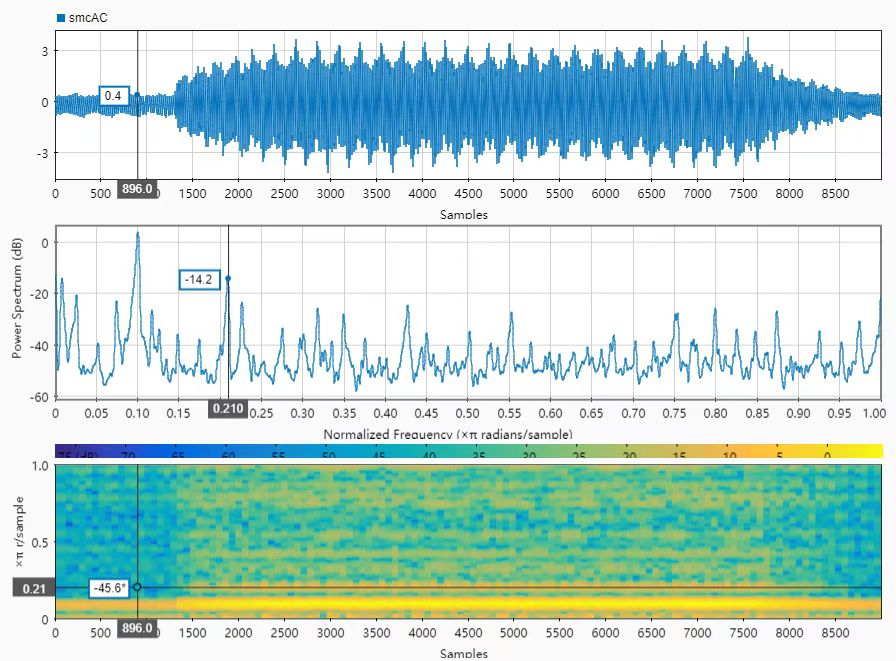
\includegraphics[width=10.5cm]{Chapter2/smcAC.jpg}
%     \caption{Matlab信号处理:以smcAC为例}
% \end{figure}
% 
% % 
% \begin{figure}[htp]
%     \centering
%     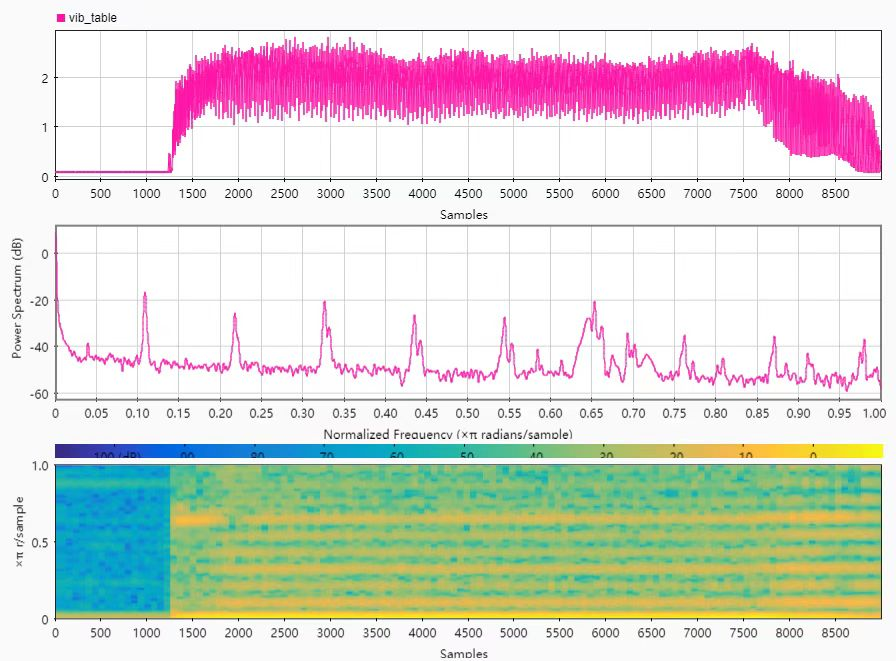
\includegraphics[width=10.5cm]{Chapter2/vib_table.jpg}
%     \caption{Matlab信号处理:vib\_table}
% \end{figure}
% % 
\begin{figure}[htbp]
% \centering
\begin{minipage}[t]{0.48\textwidth}
\centering
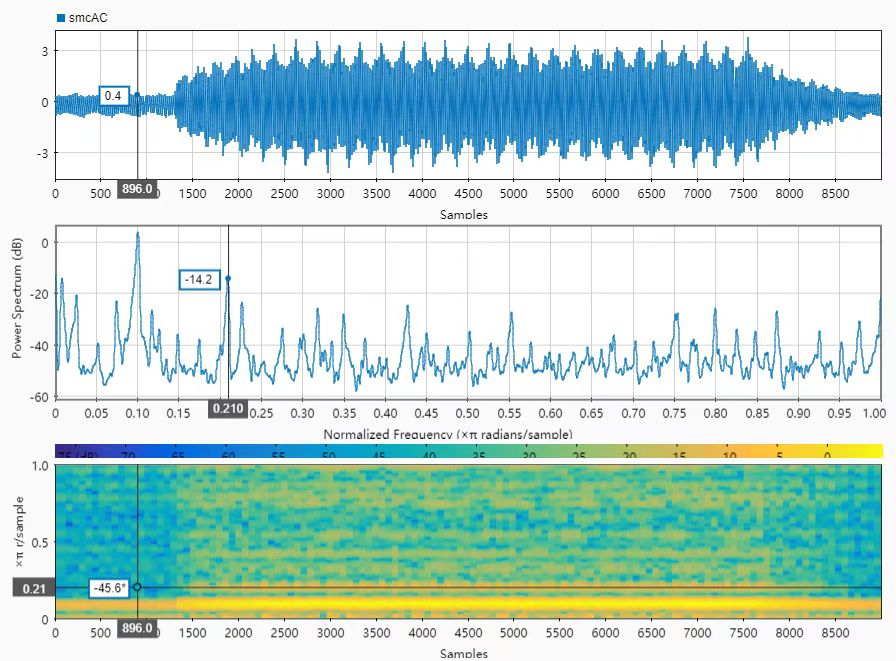
\includegraphics[width=6cm]{Chapter2/smcAC.jpg}
% \label{fig_22}
\caption{信号处理:smcAC}
\end{minipage}
\begin{minipage}[t]{0.48\textwidth}
\centering
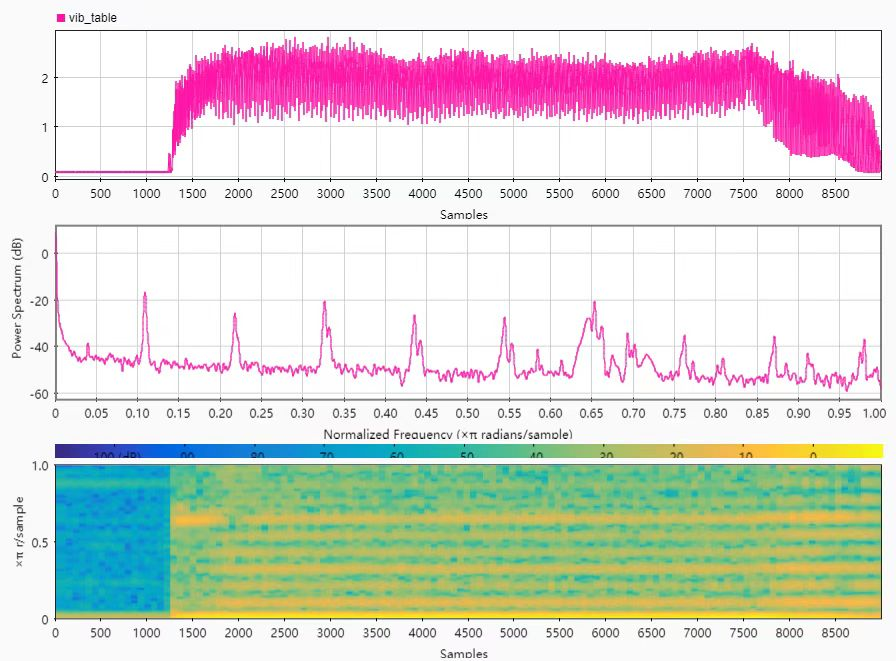
\includegraphics[width=6cm]{Chapter2/vib_table.jpg}
  \caption{信号处理:vib\_table}
% \label{fig_23}
\end{minipage}
\end{figure}

% 
\subsection{特征筛选}
如上所述,每一次的铣削过程都对应着数万条信号数据和一个真实的铣刀磨损值,但并非所有采集到的信号数据都与刀具磨损量有着相关的关系,且经过各式传感器采集得到的原始信号的数据量过于庞大,原始信号数据当中还夹杂存在着各种干扰噪声,将其直接应用于刀具磨损量分析预测会大大增大方法实现的难度。因而需要通过进行合理适当的特征工程,在海量原始信号数据当中筛选出对研究目标对象刀具磨损量较为敏感的特征。\par
%
% 
在所有高维数学和统计学问题中,对数据进行降维和特征提取都起着重要的作用。传统的变量选择方法是子集选择的方法,即从$ \left\{ \left. X_1,X_2,\cdots X_P \right\} \right. $所构成的子模型中选择其中一个。子集选择方法在p很大时计算量将变得很大,而且数据微小的变动将会导致最后结果有较大的变化。为了改进最小二乘和子集选择方法的缺点,1996年Robert Tibshirani首次提出LASSO方法。\par
LASSO方法压缩回归模型的系数,即强制令系数绝对值之和小于某个固定值,当该固定值足够小,该方法可以使得一些回归系数为零。因此同时具有子集选择和岭回归方法的优点,在处理变量很多且具有共线性的问题时,使用LASSO方法得出的结果往往具有更好的预测能力。其通过下式估计模型中的参数:\par
$$
\hat{\beta}_{Lasso}={arg\min}_{\beta \in R^{d}}\left\{ \left. \sum_{i=1}^n{\left( y_i-\beta _ix_i \right) ^2+\lambda \sum_{j=1}^p{\left| \beta _j \right|}} \right\} \right.
$$
LASSO是在RSS最小化的计算中加入一个范数作为惩罚约束。范数的好处是当λ充分大时,可以把某些待估系数精确地收缩到零。通过交叉验证法:对λ的给定值,进行交叉验证,选取交叉验证误差最小的λ值,然后按照得到的λ值,用全部数据重新拟合模型即可。\par
具体算法步骤如下所示:\par
(1)初始化$\delta _0 = sign\left( \beta ^0 \right)$,$\beta ^0$是最小二乘估计值。\par
(2)寻找$\hat{\beta}^{0}$,k表示第k次寻找,使得误差平方和$J\left( \beta \right)$达到最小。\par
$$ J\left( \beta \right) =\sum_{i=1}^{i=n}{\left( y_i-\sum_{j=1}^p{\beta _jx_{ij}^2} \right)} $$\par
(3)$\delta _0=sign\left( \beta ^0 \right) $,当$\delta _{k}^{T}\hat{\beta}^k \le t$,$\hat{\beta}^{0}$即为Lasso回归方法的最优解;否则返回步骤(2)继续寻找。\par
LASSO的优点在于,当我们惩罚参数选取的足够大时,惩罚项具有将其中较小的系数压缩为0的作用,从而可以将这些不重要的变量直接剔除,以达到特征选择的目的,因此LASSO方法特别适用于特征数目缩减与特征的选择。\par
通过建立上述特征选择分析论证得出在各通道信号中声发射信号并没有贡献出与刀具磨损量相关的最优特征,因此在本研究的实验阶段将舍弃声发射信号通道的数据。\par
% 
% 
\section{循环神经网络模型}
% 
% 
\subsection{循环神经网络模型预测训练架构}
考虑到在刀具加工工件时已经执行过前置加工任务,在使用神经网络预测刀具磨损度时若只用多层感知机模型,无法把前置隐藏状态考虑进去,因此我们使用了循环神经网络(见图2.4)。\par
\begin{figure}[htp]
    \centering
    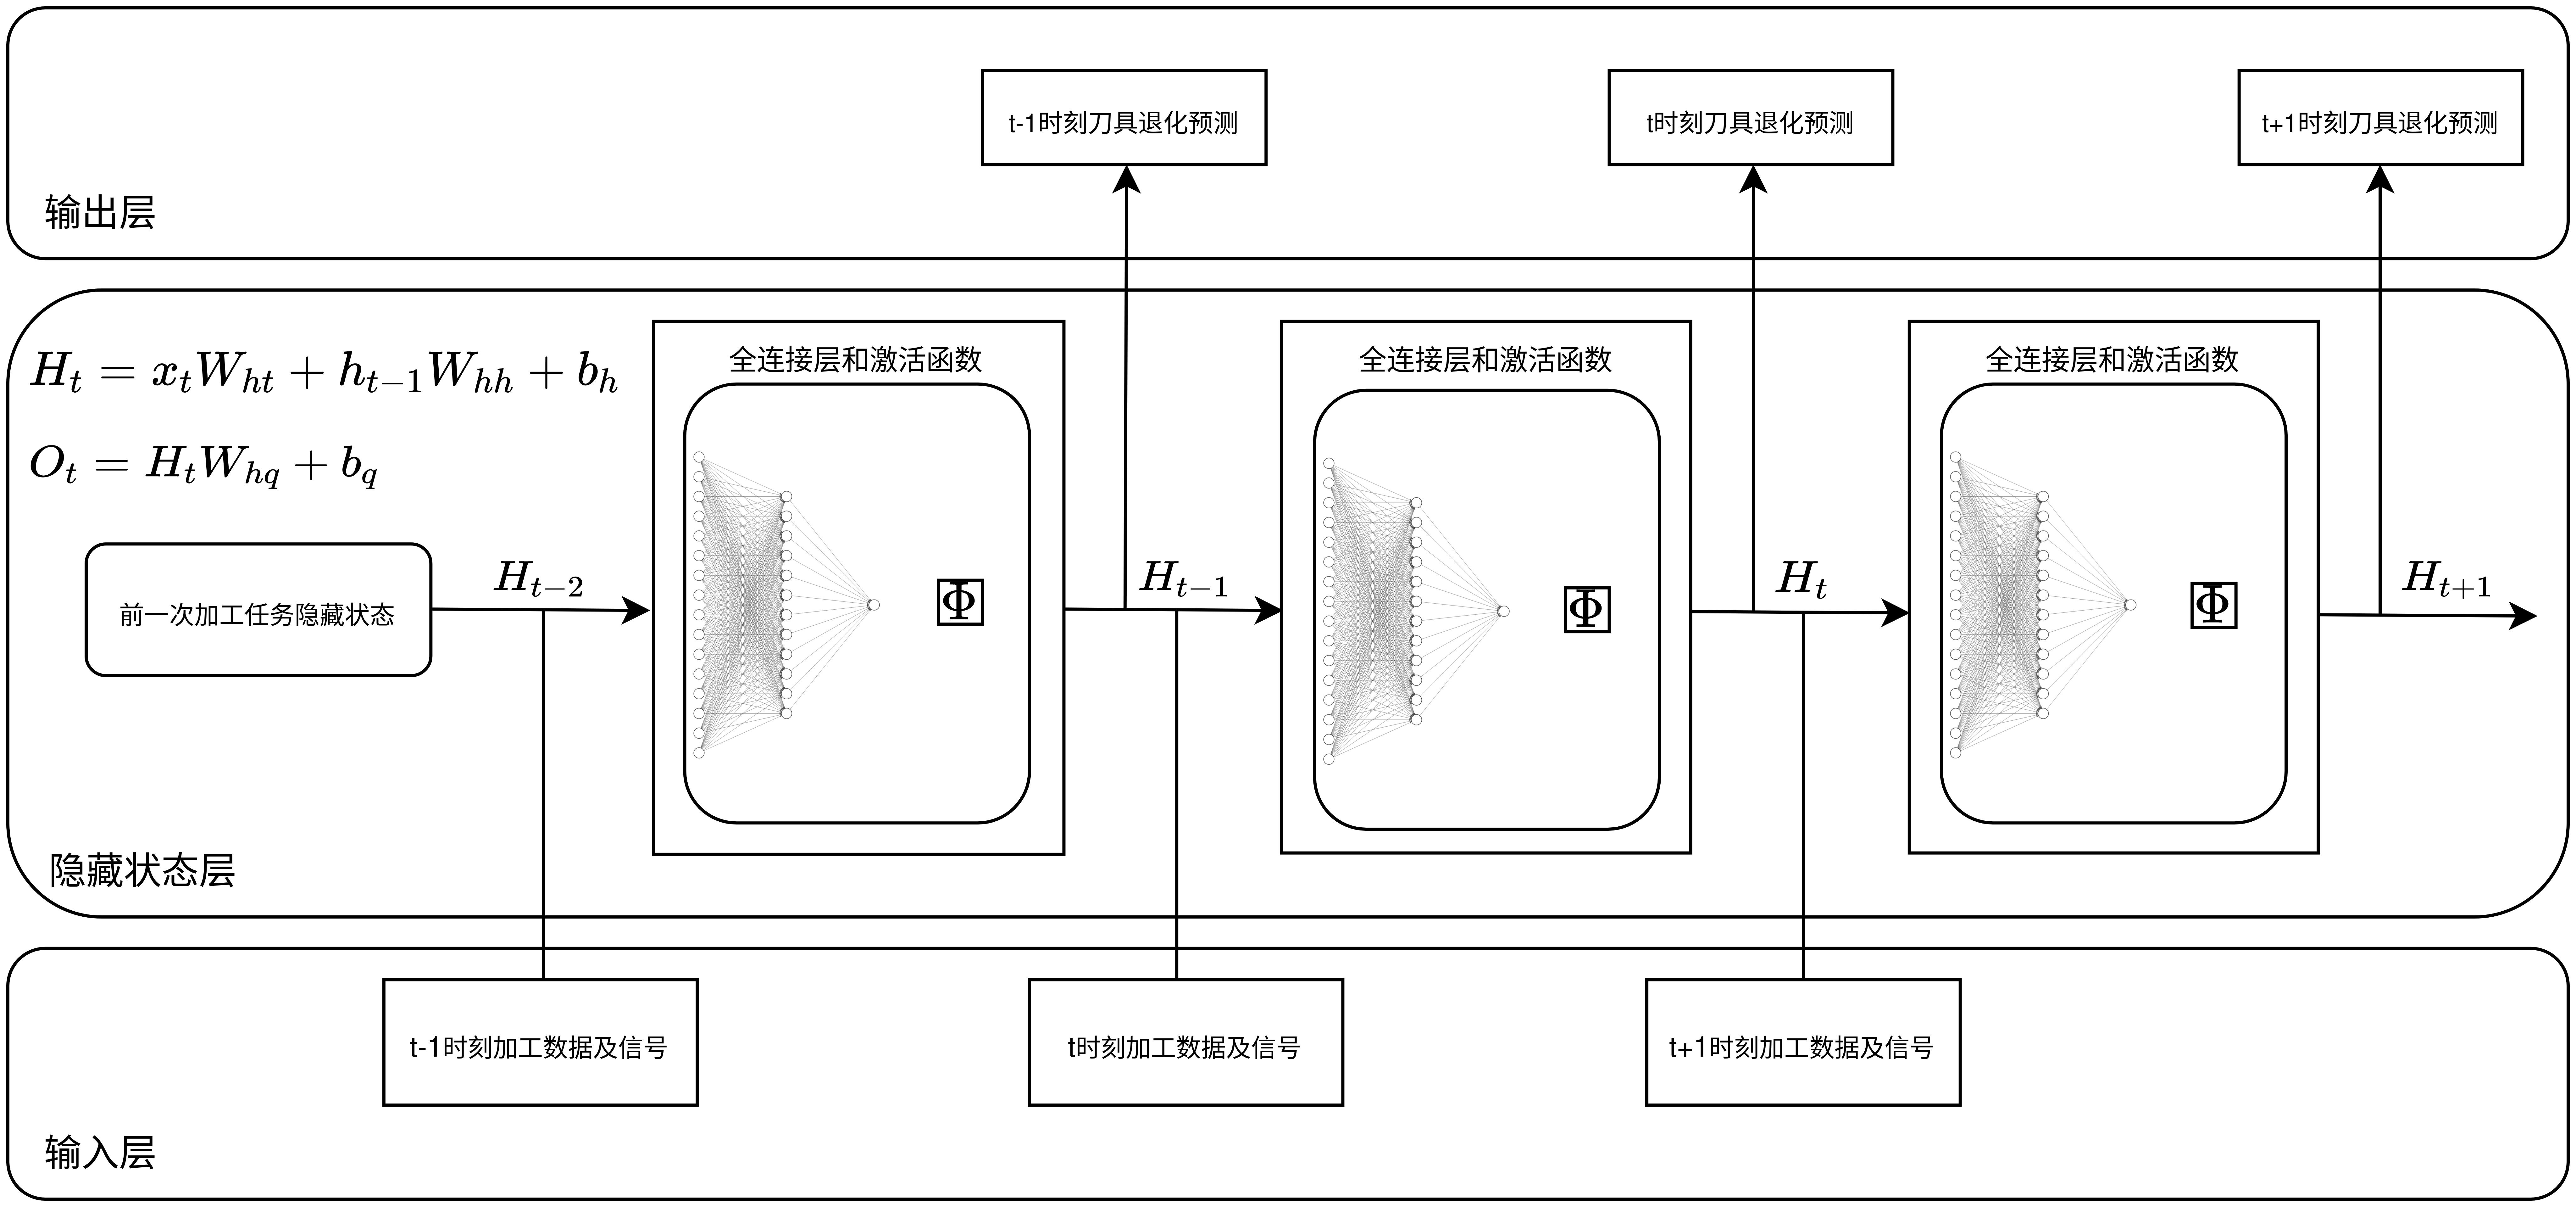
\includegraphics[width=14cm]{Chapter2/RNN architecture.png}
    \caption{机床刀具退化预测训练RNN模型}
\end{figure}
\subsection{循环神经网络模型预测训练数学展开}
输入层,输入刀具的工艺参数(进给量、加工材料、工作时长)以及经过LASSO特征筛选后的机床信号特征值作为RNN的输入:$X_t \in R^{n*d}$ ,其中n代表输入样本数量,d代表输入feature。\par
隐藏状态层,上一加工阶段的隐藏状态:$H_{t-1} \in R^{n*h}$ \par
输出层,n代表输出层输出预测值数量,与输入样本数一一对应,列代表预测值刀具退化程度:$O_t \in R^{n*1}$ \par
\subsubsection{循环神经网络迭代关系}
隐藏状态层:$H_t=\Phi(X_tW_{xh}+H_{t-1}W_{hh}+b_h)$ \par
输出层:$O_t=H_tW_{hq}+b_q$
\subsubsection{通过反向传播进行权重更新}
由于权重w和偏转变量b的值,在没有训练前是存在误差的,所以反向传播是为了找出它们的误差,并且更新它们。我们首先计算出最后一层的误差/偏导数,涉及到两个函数,一个是C损失函数,另一个是激活函数。运用数学上的偏导函数求法和导数的传递性,可以得到最后一层的误差$ \delta^{L}$。$ \delta_{j}^{L}=\frac{\partial c}{\partial a_{j}^{L}} \sigma^{\prime}\left(z^{L}\right)=\left(a_{j}^{L}-y\right) \sigma^{\prime}\left(z^{L}\right) $以此模式类推,反向求出每一层的误差/偏导数,最终可以得到关于w的误差和关于b的误差。
其反向传播公式使用步骤如下:\par
Step1 首先,使用如下公式计算出最后一层的误差\par
$$ \delta^{L}=\nabla_{a} C \odot \sigma^{\prime}\left(z^{L}\right) $$ \par
Step2 在此基础上,使用以下三个公式分别计算出倒数第二层的误差,倒数第二层关于b的误差,倒数第二层关于w的误差。\par
% $$ \begin{array}{c}
% \delta^{l}=\left(\left(w^{l+1}\right)^{T} \delta^{l+1}\right) \odot \sigma^{\prime}\left(z^{l}\right) \\
% \frac{\partial C}{\partial b_{j}^{l}}=\delta_{j}^{l} \\
% \frac{\partial C}{\partial w_{j k}^{l}}=a_{k}^{l-1} \delta_{j}^{l}
% \end{array} $$ \par
$$ \delta^{l}=\left(\left(w^{l+1}\right)^{T} \delta^{l+1}\right) \odot \sigma^{\prime}\left(z^{l}\right) $$ \par
$$ \frac{\partial C}{\partial b_{j}^{l}}=\delta_{j}^{l} $$ \par
$$ \frac{\partial C}{\partial w_{j k}^{l}}=a_{k}^{l-1} \delta_{j}^{l} $$ \par
% 
Step3 以此类推,计算到第一层,最后不断更新w和b。 \par
% \subsubsection{核心算法实现}
下方2个副加页面是基于PyTorch框架,以及本项目中对于机床刀具磨损量及输入数据构建的神经网络核心训练程序代码。
% 
% 
% 
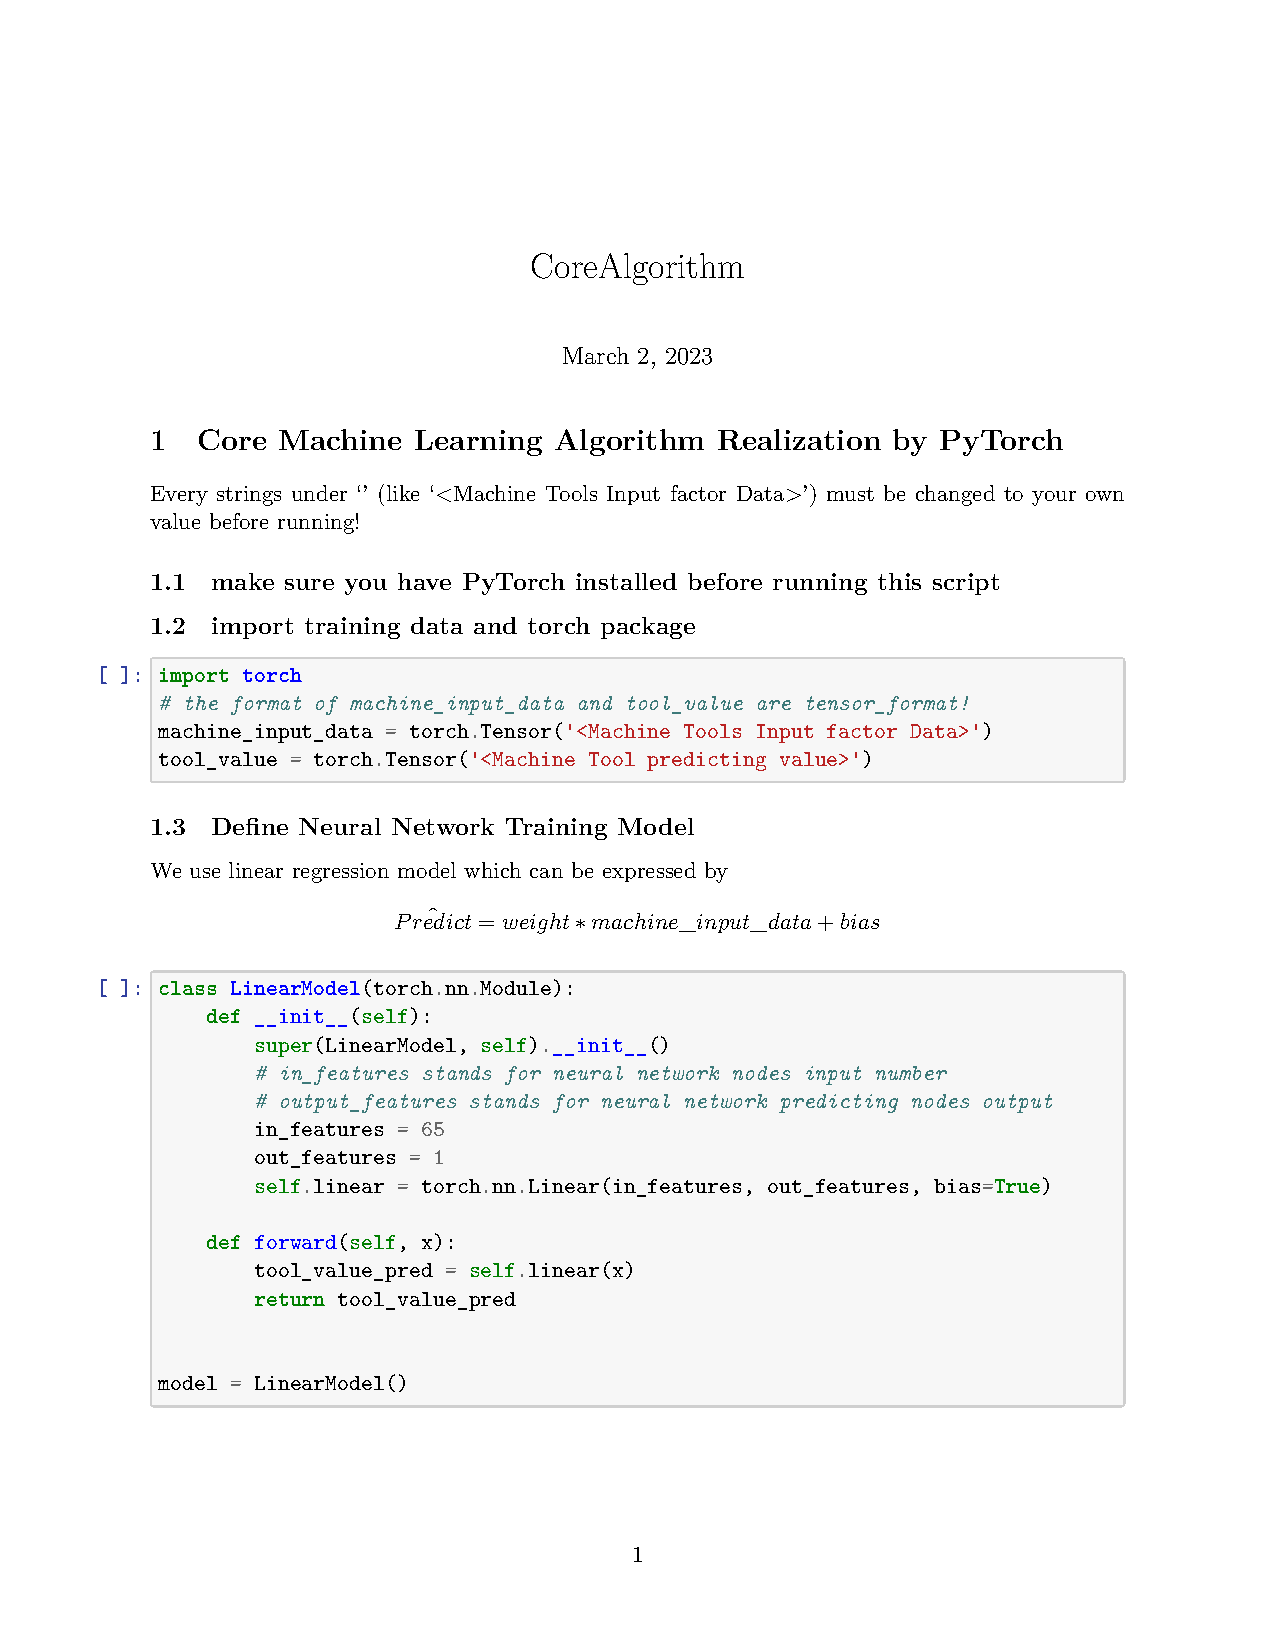
\includepdf[pages={1,2}]{Chapter2/CoreAlgorithm.pdf}
% 